\documentclass[a4paper,12pt,fleqn]{article}
\usepackage{fixltx2e}
\usepackage[utf8]{inputenc}
\usepackage{graphicx}
\usepackage{sidecap}
\usepackage{fancyhdr}
\usepackage{amssymb,amsmath}
\usepackage[swedish]{babel}
\usepackage[margin=1.5in]{geometry}
\usepackage{abstract}
\usepackage[parfill]{parskip}
\usepackage{tocloft}
\usepackage{adjustbox}
\usepackage{textcomp}
\usepackage[T1]{fontenc}
\usepackage[usenames,dvipsnames,svgnames,table]{xcolor}
\usepackage{listings}
\usepackage{hyperref}
\usepackage{tocloft}

% %% Footnotes-Listing %%
\newcommand{\listfootnotesname}{Referenser}% 'List of Footnotes' title 
\newlistof[chapter]{footnotes}{fnt}{\listfootnotesname}% New 'List of...' for footnotes 
\let\oldfootnote\footnote % Save the old \footnote{...} command 
 \renewcommand\footnote[1]{% Redefine the new footnote to also add 'List of Footnote' entries. 
     \refstepcounter{footnotes}% Add and step a reference to the footnote/counter. 
     \oldfootnote{#1}% Make a regular footnote. 
     \addcontentsline{fnt}{footnotes}{\protect 
 \numberline{\thefootnotes}#1}% Add the 'List of...' entry. 
}

%----------------------------------------------------------------
%C-kod formatering

\definecolor{listinggray}{gray}{0.9}
\definecolor{lbcolor}{rgb}{0.9,0.9,0.9}
\lstset{
backgroundcolor=\color{lbcolor},
    tabsize=4,    
%   rulecolor=,
    language=[GNU]C++,
        basicstyle=\scriptsize,
        upquote=true,
        aboveskip={1.5\baselineskip},
        columns=fixed,
        showstringspaces=false,
        extendedchars=false,
        breaklines=true,
        prebreak = \raisebox{0ex}[0ex][0ex]{\ensuremath{\hookleftarrow}},
        frame=single,
        numbers=left,
        showtabs=false,
        showspaces=false,
        showstringspaces=false,
        identifierstyle=\ttfamily,
        keywordstyle=\color[rgb]{0,0,1},
        commentstyle=\color[rgb]{0.026,0.112,0.095},
        stringstyle=\color[rgb]{0.627,0.126,0.941},
        numberstyle=\color[rgb]{0.205, 0.142, 0.73},
%        \lstdefinestyle{C++}{language=C++,style=numbers}’.
}
\lstset{
    backgroundcolor=\color{lbcolor},
    tabsize=4,
  language=C++,
  captionpos=b,
  tabsize=3,
  frame=lines,
  numbers=left,
  numberstyle=\tiny,
  numbersep=5pt,
  breaklines=true,
  showstringspaces=false,
  basicstyle=\footnotesize,
%  identifierstyle=\color{magenta},
  keywordstyle=\color[rgb]{0,0,1},
  commentstyle=\color{Darkgreen},
  stringstyle=\color{red}
  }
  %-----------------------------------------------------------------
  %marginaler

  \renewcommand{\abstractnamefont}{\normalfont\normalsize\bfseries}
  \renewcommand{\abstracttextfont}{\normalfont\small}
  \renewcommand{\headrulewidth}{0pt}
  \renewcommand{\cftsecleader}{\cftdotfill{\cftdotsep}} 
  \setlength{\absleftindent}{0pt}
  \setlength{\absrightindent}{0pt}
  \setlength{\headheight}{15pt}

  \addtolength{\oddsidemargin}{-.5in}
  	\addtolength{\evensidemargin}{-.5in}
  	\addtolength{\textwidth}{1in}


  %-----------------------------------------------------------------
  %header and footer

  \pagestyle{fancy}
  \lhead{
  	\begin{picture}(0,0)
  		\put(5,0){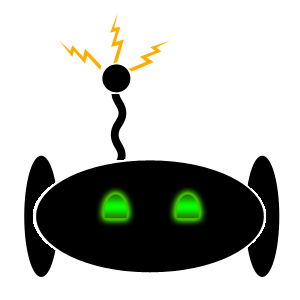
\includegraphics{logotyp.png}}
  	\end{picture}}
	
  \fancyhead[C]{\small{Mapmaster2001}}
  \fancyhead[R]{\small \today}
  \fancyfoot[L]{\small{TSEA56 \\ LIPS Kappa}}
  \fancyfoot[C]{\small{\thepage}}
  \fancyfoot[R]{\small{Projektgrupp 8 \\ mapmaster2001@cyd.liu.se}}

  %-----------------------------------------------------------------


%-------------------------------------------------------------------
%Första sidan

\begin{document}
	\pagestyle{fancy}
\pagenumbering{roman}
	\vspace*{\fill}
		\begingroup
			\begin{center}
				\huge{\textbf{Teknisk dokumentation}}
				\\
				\vspace{5pt}
				\normalsize
				Kandidatprojekt Y - Grupp 8 - VT2014
				\\
				Version 1.0
				\end{center}
		\endgroup
	 
	\vspace{15pt}
	\begin{figure}[htp] %Placera här om det finns plats, annars så snart som möjligt, på toppen av en sida.
	  \begin{center}
	  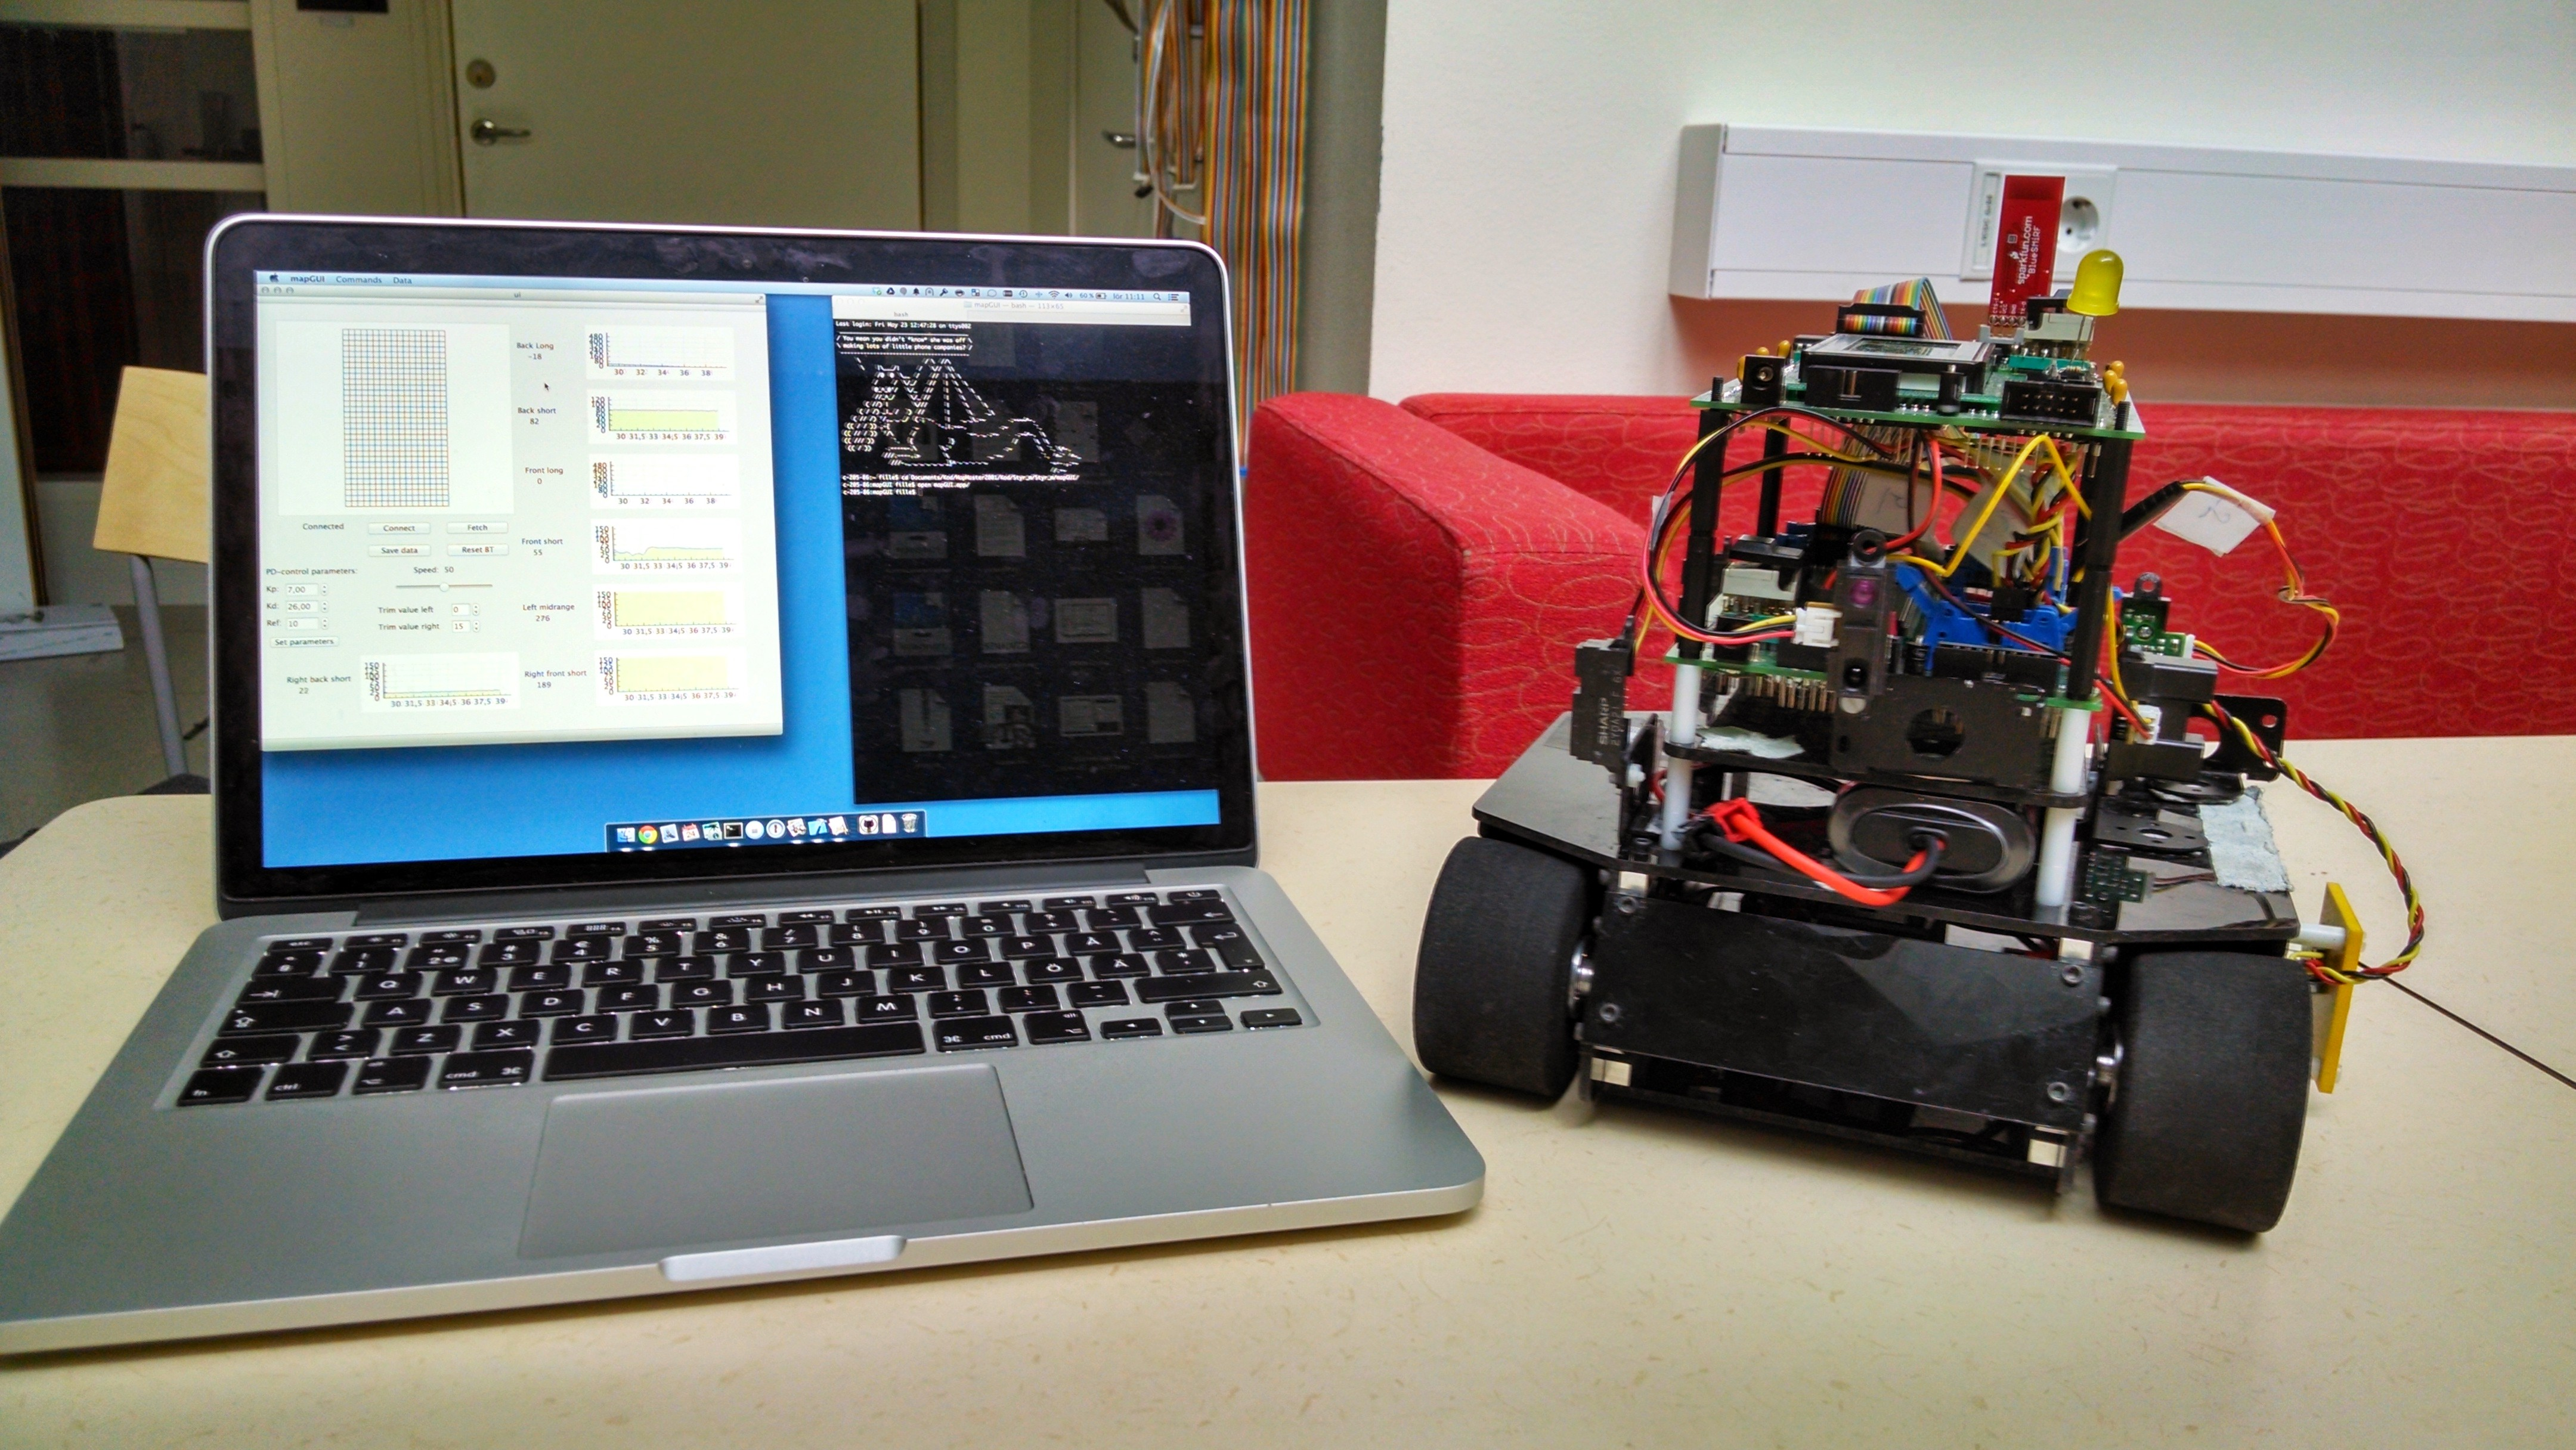
\includegraphics[keepaspectratio=true,,width=0.5\linewidth]{bilder/robotbilder/Helaroboten}
	  \end{center}
	\end{figure}
	\vspace*{\fill}
	
	\begin{center} %Börjar centrering 
		Status
		\\
		\vspace{3pt} %Whitespace 3 pts
	    \begin{tabular}{| p{3cm} | p{3cm} | p{3cm} |} %tabell, 4 horizontella |, 3 cm emellan dem.
	    \hline %översta horizontella linjen.
	    Granskad & JE,TG,HFE & \today \\ \hline % & -tecken för att "gå till nästa ruta" 
		Godkänd & - & - \\ \hline % avslutas med \\ och \hline.

	    \end{tabular}
	\end{center}
	\vspace{2cm}
	\newpage
%-----------------------------------------------------------------
%Projektidentitet
	
	\vspace*{\fill}
		\begingroup
			\begin{center}
				\LARGE{\textbf{PROJEKTIDENTITET}}
				\\
				\footnotesize
				Grupp 8, 2014/VT, MapMaster2001
				\\
				Linköpings tekniska högskola, ISY
				\\
				\vspace{1cm}
	  \begin{tabular}{| p{3cm} | p{4.3cm} | p{2.4cm} | p{3.8cm} |}
	    \hline
		\textbf{Namn} & \textbf{Ansvar} & \textbf{Telefon} & \textbf{E-post} \\ \hline
	    Jens Edhammer & Dokumentansvarig (DOK) & 076-030 67 80 & jened502@student.liu.se \\ \hline
		Erik Ekelund & Designansvarig (DES) & 073-682 43 06 & eriek984@student.liu.se \\ \hline
		David Habrman &  & 076-017 71 15 & davha227@student.liu.se \\ \hline 
		Tobias Grundström & Testansvarig (TES) & 073-830 44 45 & tobgr602@student.liu.se \\ \hline 
		Hans-Filip Elo &   & 073-385 22 32 & hanel742@student.liu.se \\ \hline 
		Niklas Ericson & Projektledare (PL) & 073-052 27 05 & niker917@student.liu.se \\ \hline
	    \end{tabular}
		
		\vspace{1cm}
		\textbf{E-postlista för hela gruppen:} mapmaster2001@cyd.liu.se
		\\[0.5cm]
		
		\textbf{Kund}: Mattias Krysander, Linköpings universitet, 581 83  LINKÖPING, \\
		013-28 21 98, matkr@isy.liu.se \\
		\textbf{Kontaktperson hos kund}: Mattias Krysander, 013-28 21 98, matkr@isy.liu.se 
		\\
		\textbf{Kursansvarig}: Tomas Svensson, 3B:528,013 28 21 59, tomass@isy.liu.se
		\\[0.5cm]
		\textbf{Handledare}: Peter Johansson, 013-28 1345, peter.a.johansson@liu.se

				\end{center}
		\endgroup
	\vspace*{\fill}
\newpage

%-----------------------------------------------------------------
%Innehållsföreteckning

\addto\captionsswedish{\renewcommand{\contentsname}{Innehållsförteckning}}

\tableofcontents
\newpage
\listoffigures
\thispagestyle{fancy}
\newpage

\pagenumbering{arabic}

%-----------------------------------------------------------------
%Översikt

\section{Tidsåtgång}
\subsection{Arbetsfördelning}
\subsection{Tidsåtgång jämfört med planerad tid}
\section{Analys av arbete och problem}
\subsection{Vad hände under de olika faserna (bra/dåligt/orsak)}
\subsection{Hur använde vi projektmodellen}
\subsection{Hur fungerade relationen med beställaren?}
\subsection{Hur fungerade relationen med handledaren?}
\subsection{Tekniska framgångar/problem}
%Beskriv de 3 besvärligaste problemen som ni har haft under projektet. 
%Rangordna problemen där 1 är mest besvärlig i betydelsen tog längst tid att fixa.
%Beskriv för varje problem:
%a. felets typ - ange t.ex.  hårdvarufel, mjukvarufel, systemintegrationsfel 
%b. kort beskrivning av felets symptom 
%c. kort beskrivning av felets orsak t.ex. logiskt fel i programmering, timing-fel, %glappkontakt, missförstånd av spec., felaktig design. 
%d. kort beskrivning av hur ni fixade felet. T.ex. hur ni fixade mjukvarubuggen, fick ny %hårdvara, virade om, gick runt problemet.
%e. ungefärlig skattning av hur mycket tid som ni ägnade åt felsökningen (dvs. tid som kunde tjänats in om felet inte hade uppstått)

\section{Måluppfyllelse}
\subsection{Vad har uppnåtts?}
\subsection{Hur fungerade leveransen?}
\subsection{Hur har studiesituationen påverkat projektet?}
\section{Sammanfattning}
\subsection{De tre viktigaste erfarenheterna}
\subsection{Goda råd till de som ska utföra ett liknande projekt}s 



\end{document}
